\documentclass{article}

% if you need to pass options to natbib, use, e.g.:
% \PassOptionsToPackage{numbers, compress}{natbib}
% before loading nips_2016
%
% to avoid loading the natbib package, add option nonatbib:
% \usepackage[nonatbib]{nips_2016}

\usepackage{nips_2016}

% to compile a camera-ready version, add the [final] option, e.g.:
% \usepackage[final]{nips_2016}

\usepackage[utf8]{inputenc} % allow utf-8 input
\usepackage[T1]{fontenc}    % use 8-bit T1 fonts
\usepackage{hyperref}       % hyperlinks
\usepackage{url}            % simple URL typesetting
\usepackage{booktabs}       % professional-quality tables
\usepackage{amsfonts}       % blackboard math symbols
\usepackage{nicefrac}       % compact symbols for 1/2, etc.
\usepackage{microtype}      % microtypography
\usepackage{graphicx,color}
\usepackage{listings}

\newcommand{\todo}[1]{\textcolor{blue}{#1}}

\title{Group S15: Mini Project Report}

% The \author macro works with any number of authors. There are two
% commands used to separate the names and addresses of multiple
% authors: \And and \AND.
%
% Using \And between authors leaves it to LaTeX to determine where to
% break the lines. Using \AND forces a line break at that point. So,
% if LaTeX puts 3 of 4 authors names on the first line, and the last
% on the second line, try using \AND instead of \And before the third
% author name.

\author{
  Petar Bokan \\
  \texttt{petar.bokan@physics.uu.se} \\
  %% examples of more authors
   \And
  Pavol Bauer \\
  \texttt{pavol.bauer@it.uu.se} \\
}

%add lines according to instructions
\makeatletter
\renewcommand{\@noticestring}{}
\makeatother

\begin{document}
% \nipsfinalcopy is no longer used

\maketitle

\begin{abstract}
Supervised machine learning methods such as regression, random forest and boosting gained enormous importance in research as well as industrial applications.
We consider a problem classifying favourite songs based on a feature dataset obtained from a streaming music company.
We train and validate the random forest and boosting classifiers and test their performance on a unknown test set.

\end{abstract}

\section{Introduction}

In this miniproject we implement, validate, and benchmark two classification methods used in statistical machine learning; random forests and boosting.
We consider a training dataset of 400 songs that can be classified into two categories based on 13 features (Figure \ref{fig:pairs}).
After training the classifiers on the dataset, we evaluate their performance on a test dataset consisting of 100 songs.
The prediction of the test data is evaluated using a web-based platform, which returns the percentage of successfully classified songs.

\begin{figure}[htp!]
  \centering
  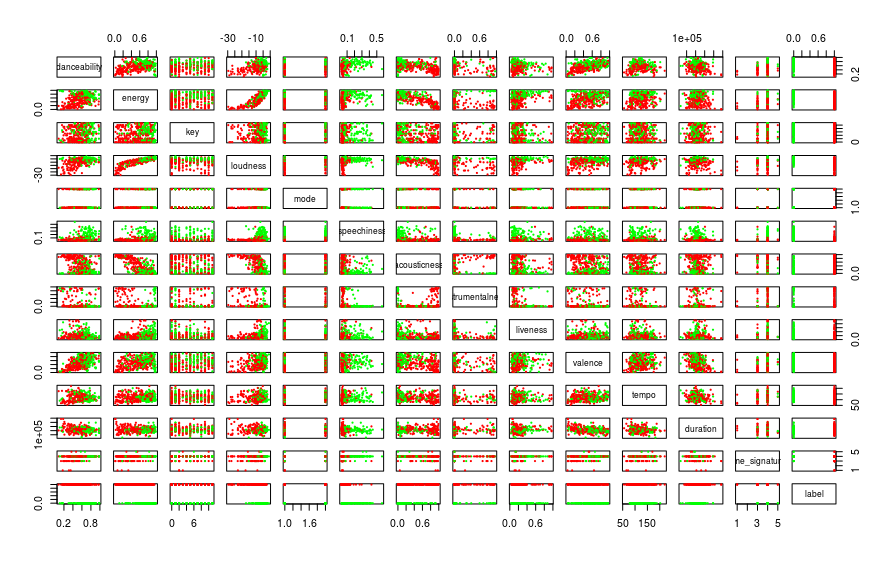
\includegraphics[height=0.5\textwidth] {figs/song_pairs.png}
  \caption{The trainig data set consists of 400 songs that are classified in 2 categories, ``liked'' (red dots) and ``disliked'' (green dots), based on 13 features.}
  \label{fig:pairs}
\end{figure}

\section{Methods}

\subsection{Random Forest}

Random Forest belongs to the family of tree-based methods, which rely on the training and evaluation of decision trees.
Decision trees are built by segmenting the predictor space into a number of regions, typically using a technique called \textit{recursive binary splitting}.
For classification, each region of the tree is assigned to a predictor class.
A point that falls into the region is straightforwardly classified as belonging to the class.

\textit{Bagging} makes use of a statistical technique called Bootstrap. 
Bootstrapping is a test that allows to estimate sample metrics such as bias and variance using random sampling with replacement.
Typically, decision trees suffer from high variance, depending on which part of the training data they have been built [1].
The idea of bagging is than to sample the training data with replacement, and creating $B$ bootstrapped sets $\hat{f}^{*b}$. 
The bagged predictor is than computed by the average of the bootstrapped sets,

\begin{equation} \label{boost_error_rate}
\hat{f}_{bag}(x)=\frac{1}{B}\sum_{b=1}^{B}\hat{f}^{*b}(x),
\end{equation}

and has a provably lower variance than an individual decision tree [1].

\textit{Random Forests} further decorrelate the ensemble of bagged trees by considering only a random subset of predictors instead of the complete set. As a rule of thumb, the method takes $m \sim  \sqrt{p}$ predictors at each split, where $p$ is the total amount of predictors. This increases the variance of trees as, for example, strong predictors that otherwise would be correlated in all of the trees, are now left out. 

\subsection{Boosting}

Boosting [1,2] is one more technique that can be used for improving the predictions resulting from a decision tree. Originally it was designed for improving classification methods, but soon it was realized that it can be applied to many statistical learning methods, both for classification and regression problems. It is considered to be one of the most successful machine learning ideas.

Weak models, those models that perform only slightly better compared to random guessing, are built sequentially. In this series of week models, each one tries to correct the mistakes made by the previous one. Eventually, they are all combined into final, much stronger, model. 

Classification problem discussed in this report is a two-class problem. For building boosting decision tree binary classifier $G(x)$, ``AdaBoost'' algorithm, which is one of the oldest and the most popular boosting algorithm, will be used. The output of this classifier will tell us if the classifier predicts that Andreas likes the specific song, or that he does not like it, for each song in data set. The classification tree is sequentially applied to repeatedly modified versions of data, producing a sequence of week classifiers $G_m(x)$, $m=1,2,...,M$. The error rate on the training sample is:

\begin{equation} \label{boost_error_rate}
\bar{err}=\frac{1}{N}\sum_{i=1}^{N}I(y_i\neq G(x_i)).
\end{equation}

These week classifiers, with output coded as $\left\{-1,1\right\}$, are combined through a weighted
majority vote to produce the final prediction:

\begin{equation} \label{boost_final_pred}
G(x)=sign(\sum_{m=1}^{M}\alpha_m G_m(x)).
\end{equation}

\section{Implementation}

\subsection{Random Forest}

For the random forest classification we used the R-package {\fontfamily{cmtt}\selectfont randomForest}. The call has a set of parameters which are important to consider. Relevant for our application, {\fontfamily{cmtt}\selectfont ntrees} determines the number of trees to grow. This should not be a small number to ensure that every input rows gets predicted at least a few times.
An other important variables is {\fontfamily{cmtt}\selectfont mtry}, which determines the number of variables that are randomly sampled as candidates at each split. Here we used the default split size $m=\sqrt{p}$, which was discussed previously.

We carried out k-fold cross-validation for feature selection using the {\fontfamily{cmtt}\selectfont rfcv} command, which makes use of the algorithm described by [4].  The algortihm varies the importance measure for all predictors and potentially tries to remove irrelevant variables. The algortihm has the following structure:
\begin{enumerate}
\item Partition the data for 5-fold cross-validation (CV).
\item On each CV training set, train a model on all variables and use the variable
importance measure to rank them. Record the CV test set predictions.
\item Use the variable ranking to remove the least important half of the variables
and retrain the model, predicting the CV test set. Repeat removal of half of
the variables until there are about 2 left.
\item Aggregate results from all 5 CV partitions and compute the error rate (in
classification) or mean squared error (in regression) at each step of halving.
\item Replicate steps (1)-(4) 20 times to “smooth out” the variability.
\end{enumerate}

\subsection{Boosting}

For the classification problem discussed in this report we also applied boosting classification tree method. AdaBoost is available in R as the command {\fontfamily{cmtt}\selectfont boosting} in the {\fontfamily{cmtt}\selectfont adabag} package [3].

There are several parameters that need to be optimized. The parameter {\fontfamily{cmtt}\selectfont mfinal} represents the number of trees (weak classifiers) that is used to build the final model. Boosting can overfit if the value of this parameter is too large. Default value is $100$. The parameter {\fontfamily{cmtt}\selectfont maxdepth} sets the maximum depth of any node of the final tree. The root node is counted as $0$. If not specified it will be set equal to the number of classes. The {\fontfamily{cmtt}\selectfont minsplit} value defines the minimal number of observations (data points) that each node needs to have in order for a further split to be attempted. The complexity parameter {\fontfamily{cmtt}\selectfont cp} tells us how much the overall performance of a fit has to be improved by a given split in order for it to happen. All these parameters were optimized while constructing the model. Parameters {\fontfamily{cmtt}\selectfont maxdepth}, {\fontfamily{cmtt}\selectfont minsplit} and {\fontfamily{cmtt}\selectfont cp} were implemented through {\fontfamily{cmtt}\selectfont control} option of a {\fontfamily{cmtt}\selectfont boosting} command.

We use $K-$fold cross-validation to get the confusion matrix for the data set. Since number of unlabeled songs is $100$, we will use $4-$fold cross-validation for our $400$ songs data set. This is implemented using {\fontfamily{cmtt}\selectfont boosting.cv} command. The data is split into $4$ subsets. One of these subsets is used to asses the performance of our prediction model, while other subsets are used as training data. The procedure is repeated for all possible combinations.

\section{Validation}

\subsection{Random Forest}

We first computed the cross-validation for variable selection, that is described in the previous section.
As the method relies on a random seed which determines how trees are generated, we repeated the cross-validation $N=10$ times and computed a mean and standard deviation of the test error.
As shown in Figure~\ref{fig:numpredictors}, for more than 5 predictors the test-error lies within a similar margin.
However, the mean value is lowest for the case where all the predictor values are considered.

\begin{figure}[htp!]
  \centering
  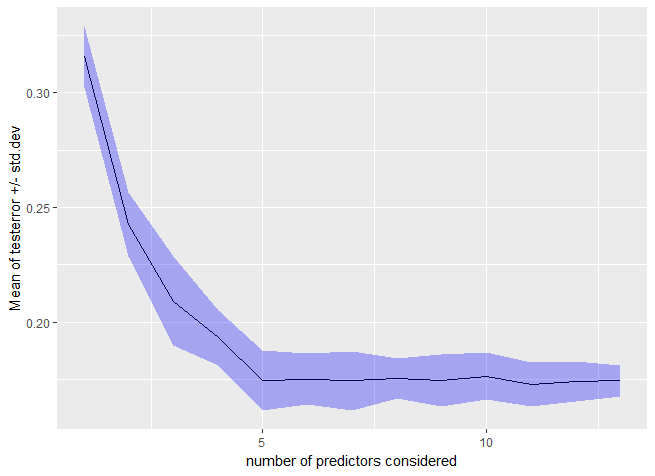
\includegraphics[height=0.5\textwidth] {figs/numpredictors.png}
  \caption{Varying the number of predictors considered (N=10).}
  \label{fig:numpredictors}
\end{figure}

Likewise, we evaluated the impact of the tree size on the test error, which is depicted in Figure~\ref{fig:treesize}.
Here we have splitted the data into a training and validation part, with a ratio of $0.75:0.25$, and re-sampled the dataset $N=40$ times for a different choice of bootstraps $B$.
We found that as long as $B$ is larger than 30, the test error lies within the same margin.
Note, that the test error is strongly varying depending on the split of the dataset, with a standard deviation of more than $5\%$.

This result motivated us to use all predictors and a large choice of $B$ for classification of the test data.

\begin{figure}[htp!]
  \centering
  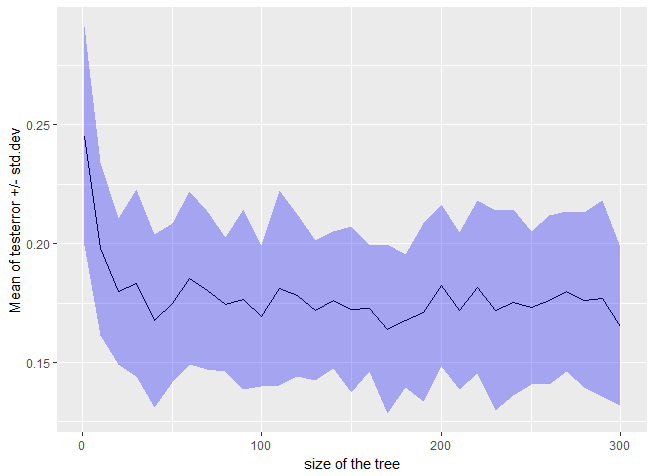
\includegraphics[height=0.5\textwidth] {figs/treesize.png}
  \caption{Varying the number of generated trees (N=40).}
  \label{fig:treesize}
\end{figure}

\subsection{Boosting}

Initially, data set of $400$ songs was randomly divided into a training data set and a test data set consisting of $300$ and $100$ songs, respectively. 

A boosted classification tree model was build for several different values of complexity parameter. In Figure \ref{fig:complexity_parameter_values} we see how prediction error changes for different values of this parameter. Conclusion is that there is no clear dependence, but still, the minimal improvement of an overall fit performance, for a given split to be done, should not be to low, since this leads to overfitting. For further parameter optimization we keep {\fontfamily{cmtt}\selectfont cp$=0.01$} fixed.
 
 \begin{figure}[h] %b-dole, t-gore, h-here,
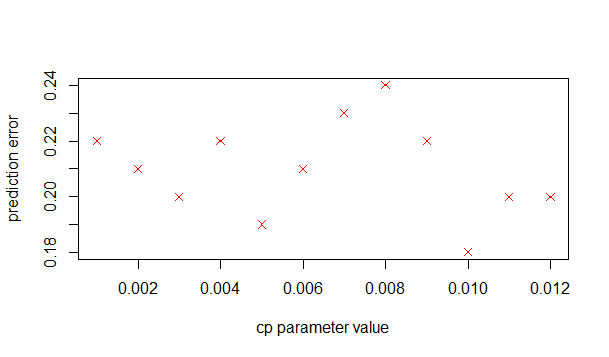
\includegraphics[scale=0.65]{figs/cp_values.png}
\centering
\caption{Prediction error for different complexity parameter values.} \label{fig:complexity_parameter_values}
\end{figure}
 
 We also see that there is no clear dependence between prediction error and {\fontfamily{cmtt}\selectfont maxdepth} parameter value. This is shown in Figure \ref{fig:maxdepth_parameter_values}. We use fixed value {\fontfamily{cmtt}\selectfont maxdepth$=7$}. Next in our list is a {\fontfamily{cmtt}\selectfont minsplit} parameter and the conclusions here are similar. There is no obvious trend.
 
\begin{figure}[h] %b-dole, t-gore, h-here,
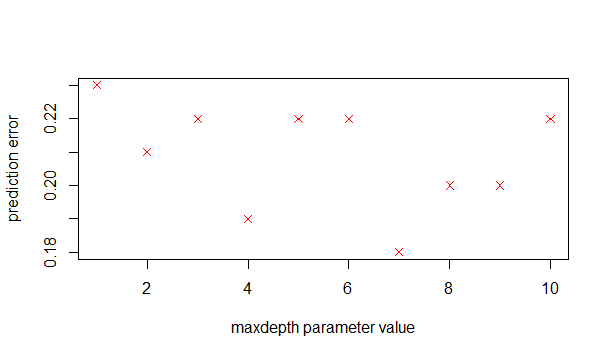
\includegraphics[scale=0.65]{figs/maxdepth_values}
\centering
\caption{Prediction error for different {\fontfamily{cmtt}\selectfont maxdepth} parameter values.} \label{fig:maxdepth_parameter_values}
\end{figure}

Figure \ref{fig:mfinal_parameter_values} shows how ensemble error changes while number of trees in a model grows. It looks like there is no overfitting, but we also see that lower values of parameter {\fontfamily{cmtt}\selectfont mfinal} can be used and good performance will still be achieved. We use {\fontfamily{cmtt}\selectfont mfinal$=50$} trees.

\begin{figure}[h] %b-dole, t-gore, h-here,
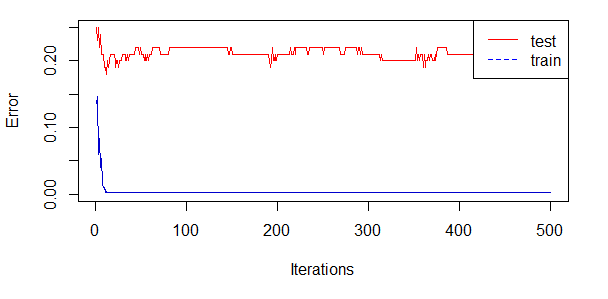
\includegraphics[scale=0.65]{figs/mfinal_500}
\centering
\caption{Ensamble error vs number of trees in a model} \label{fig:mfinal_parameter_values}
\end{figure} 

As explained, we use $4-$fold cross-validation to get the confusion matrix for the data set. Result is given in Table \ref{tab:confussion_matrix}. Prediction error in this case is below $0.20$, so we can conclude that the model is independent of our training$/$test data set definition, since the results are consistent.

\begin {table}[h]
\begin{center}
\begin{tabular}{r|r|r}
  Observed & 0  & 1 \\
  \hline			
  Predicted 0 & 107 & 32 \\
  1 & 46 & 215 \\ 
\end{tabular}
\end{center}
\caption {$4-$fold confussion matrix. $0-$Andres did not like the song; $1-$Andreas liked the song.} 
\label{tab:confussion_matrix} 
\end {table}

\section{Results}

The performance of the presented methods obtained on the training dataset is shown in Table \ref{tab:performance}.
The naive classifier classifies all points of the test dataset as ``like''.

\begin {table}[h]
\begin{center}
\begin{tabular}{r|r}
  Method & Performance   \\
  \hline			
  Boosting & 84 \% \\
  Random Forest & 80 \% \\
  Naive & 60 \%
\end{tabular}
\end{center}
\caption {Performance of our classifiers on the test dataset.} 
\label{tab:performance} 
\end {table}

\section{Conclusion}

In this mini-project we used two supervised machine learning methods to classify a set of song data into like and disliked songs.
We implemented, validated, and evaluated two methods; random forests and boosting.

We have implemented and validated the random forest method and found that it is strongly sensitive to the used training data. During the cross-validation procedure we have shown that the validation error can vary within a standard deviation of $5\%$, depending solely on the split of training and validation data. This variance, that is possibly a consequence of the small data size,  also prohibited the fine-tuning the method to specific parameter ranges. However, the method performed reasonably well on the test dataset using the default parameter settings.

We showed that boosting classification tree method performs very well after simple tuning. It was seen that there is no visible dependence between the prediction error and some of the fit parameters. It might be that our data set was simply not large enough to be sensitive to variations of some of the parameters.


\section{Contributions}

So far anonymized.

%Petar implemented and validated the Boosting Method.
%Pavol implemented and validated the Random Forest Method.
%The report was written jointly by both authors.

\section*{References}

\small

[1] Hastie, T., Tibshirani, R. \ \& Friedman, J., (2008) {\it The Elements of Statistical Learning: Data Mining, Inference, and Prediction}, Springer, New York.

[2] James, G., Witten, D., Hastie, T. \ \& Tibshirani, R., (2013) {\it An Introduction to Statistical Learning
with Applications in R}, Springer, New York.

[3] Alfaro, E., Gamez, M. \ \$ Garcia, N., with contributions from Li, G. \ (2015) {\it Multiclass AdaBoost.M1, SAMME and Bagging Version 4.1}

[4] Svetnik, V., Liaw, A., Tong, C. \ \& Wang, T., \ (2014) {\it Application of Breiman’s Random Forest to Modeling  Structure-Activity  Relationships  of  Pharmaceutical  Molecules}

\appendix

\section{Code: random forest}

\lstinputlisting[language=R]{code/miniproject_rf.R}
\lstinputlisting[language=R]{code/colVars.R}

\section{Code: boosting}
\lstinputlisting[language=R, breaklines=true]{code/boosting.R}
\end{document}
